% AER-Article.tex for AEA last revised 22 June 2011

% \documentclass[AER]{AEA} modified for the full path to my AEA.cls file
    \documentclass[AER]{./aea-latex-templates/AEA}

        \usepackage{tikz}
        \usetikzlibrary{calc,matrix}
        
        % The mathtime package uses a Times font instead of Computer Modern.
        % Uncomment the line below if you wish to use the mathtime package:
        % \usepackage[cmbold]{mathtime}
        % Note that miktex, by default, configures the mathtime package to use commercial fonts
        % which you may not have. If you would like to use mathtime but you are seeing error
        % messages about missing fonts (mtex.pfb, mtsy.pfb, or rmtmi.pfb) then please see
        % the technical support document at 
        % for instructions on fixing this problem.
        
        % harvard for bibtex, recommended by AEA
        \usepackage[abbr]{harvard}
        % booktabs for tables, recommended by https://tex.stackexchange.com/a/59035/197312
        \usepackage{booktabs}
        
        % This command determines the leading (vertical space between lines) in draft mode
        % with 1.5 corresponding to "double" spacing.
        \draftSpacing{1.5}
        
        % allowing images as figures
        % ref: https://tex.stackexchange.com/questions/19176/how-to-insert-an-image-into-latex-document
        \usepackage{graphicx}
        \graphicspath{{./figures-and-tables}}
        
        \usepackage{hyperref}
        
        \begin{document}
        
        \title{Attitudinal Trends in Alternative Postsecondary Learning
            \thanks{
                Go to \url{https://papers.ssrn.com/sol3/papers.cfm?abstract_id=3387110} to visit
                the article page for additional materials including the online appendix,
                survey data, and data analysis source code.
            }
        }
        \shortTitle{Trends in Alternative Learning}
        \author{John Vandivier
            \thanks{
                    Vandivier: George Mason University,
                    4400 University Dr, Fairfax, VA 22030,
                    jvandivi@masonlive.gmu.edu.
                    The author acknowledges valuable input from Bryan Caplan at George Mason University.
                }
            }
        \date{\today}
        \pubMonth{Month}
        \pubYear{Year}
        \pubVolume{Vol}
        \pubIssue{Issue}
        \JEL{D12, I21, I22, I24, I25, I26}
        \Keywords{Education economics, alternative education, debt crisis, signaling}

        \begin{abstract}
        This paper explores a novel data set (n = 1190) to understand trends in public
        disposition on alternative postsecondary learning, with a focus on employers.
        Results indicate that public favorability is positive and will remain flat over the next year.
        Employer attitudes are not meaningfully different from the general public.
        \end{abstract}

        \maketitle
        
        \section{Introduction}

        Student loan debt in the United States is the highest ever\cite{friedman2018student},
        even while accredited postsecondary education is becoming a dynamically worse investment
        for at least two reasons.

        The first reason is the plain fact that college is growing in price while adjusted return remains stagnant.
        From 1989 to 2012, K-12 student expenditure increased significantly
        \footnote{
            From 1989 to 2012, the average cost of a year of undergraduate education in the US rose 79 percent
            from \$11,862 to \$21,222 in constant 2016 dollars.
            This price includes tuition and fees plus room and board for full-time students in degree-granting postsecondary institutions.
            Data from \cite{nces2017averageundergraduatetuition}.
        },
        the cost of a year of undergraduate education grew nearly three times more quickly than that
        \footnote{
            From 1989 to 2012, per pupil public expenditure for K-12 students increased 27 percent
            from \$8,654 to \$11,011 in constant 2014 dollars. Data from \cite{nces2015expendituresperpupil}.
        },
        and the adjusted average starting salary of a college graduate decreased by about 9 percent
        \footnote{
            From 1989 to 2012, a decrease of \$4,385 from \$49,487 to \$45,102 in constant 2016 dollars is observed. (4385/49487) = 0.089.
            From 1960 to 2012, an increase from \$47,442 to \$50,219 is observed. Data from \cite{koncz2016}.
        }.

        The second reason traditional postsecondary education has become a
        weaker investment during recent years is the growth of alternatives.
        This paper fills an empirical gap in scholarly research by supplying
        systematic and general data about public and employer favorability of
        alternative credentials.
        This paper tests the hypothesis that employer favorability is positive toward alternative credentials.
        % Alternative education faces adoption problems among learners, employers,
        % and third parties such as parents and teachers which influence the former two groups.
        % Learner willingness to consume alternative education is endogenous with employer favorability and entry-level job suitability.
        % If employers are favorable, dispersion of favorability information would at once explain the growth of alternative education and also ostensibly stimulate further adoption.
        
        Alternative postsecondary learning activities are diverse and do not
        exclude attainment of an accredited degree, but may involve strategic
        delay or acceleration of accredited education when compared to traditional approaches.
        Delayed formal education improves the return to education for
        individuals who are able to leverage employer funding. Accelerated completion improves the return to education in general.
        Online education is an alternative approach which reduces the cost of college for most students
        \footnote{
            Mattern and Wyatt\cite{mattern2009student} note that college students live an average distance of
            268 miles from home and a median of 94 miles. This indicates that most students could reduce
            the cost of college by studying remotely from home.
        }.
        
        \section{Data}
        
        1190 responses, including partial responses, were obtained for four
        comparable survey administrations from February 2018 to May 2019.
        Analysis includes 114 right-hand variables and two left-hand variables.
        Appendix A details the wording of questions and possible responses.
        Appendix B identifies factors included in each administration.

        Responses were collected mainly through SurveyMonkey and Amazon Mechanical
        Turk paid response, with a non-trivial number also coming from social media
        and word of mouth. Each origination channel was grouped using a construct
        called a collector. Collector effects were insignificant. This is
        interesting for two reasons. First, the source
        populations are known to be systematically different. Amazon Mechanical Turk
        respondents, for example, were guaranteed to be U.S. High School graduates. A second
        reason the insignificance of collector effects is important is that
        response prices were significantly different. Amazon Mechanical Turk
        responses were more than 20 percent cheaper than SurveyMonkey Paid Audience
        responses on average.
        
        Factor-level sample size ranges from 240 to 1190. Appendix C lists
        technical variable names in alphabetical order along with summary
        statistics. Appendix D lists variable names in alphabetical order, and
        summarizes factor strength across models.
        Several constructs, such as income, age, and gender, were redundantly
        operationalized using different measures. For example, age was measured
        continuously and also by age group. Appendix D makes this
        factor-to-variable mapping clear.
        
        The variable of interest is entry-level suitability.
        This variable corresponds to question 2 in Appendix A.
        It is structured as a favorability question on a scale from 1 to 10. Higher numbers indicates stronger agreement.
        The wording of the statement to be favored is, "For many professions, alternative credentials can qualify a person for an entry-level position."
        
        A secondary variable of interest explored is called the index of interest.
        This is a 3-factor index of similar but different favorability questions.
        This variable was checked to ensure findings are robust to the specic wording of the primary variable of interest.
        This variable also includes a question on online learning. As a result, findings are more broadly generalizable
        to alternative education, rather than alternative credentials in particular.
        
        No survey administration allowed for measurement of all variables simultaneously,
        but within each calender year ordinary least squares modelling identified four key models.
        Analysis of survey results from 2018 indicated that certain factors were unimportant.
        As a result, some questions were replaced in 2019.

        The 2019 analysis covers the whole data set, not only samples from 2019.
        Questions in the October 2018 administration are a superset of those in February 2018.
        Similarly, May 2019 variables are a superset of February 2019.
        It turns out that the most significant factors identified in the
        2019 analysis were also measured in the 2018 administrations, but this may be due to oversampling.
        
        The first key model is a long model using all available right hand variables.
        Factors are eliminated one at a time until a subsequent key model is obtained.
        The second key model is the weak model. This model includes factors with a p-value of less than .5.
        The third model is an adjusted r-squared maximizing model, and the fourth
        model is a strong model involving factors with a p-value less than .1.

        \section{Empirical analysis and results}

        The average response for the variable of interest was 6.61.
        The median response was 7 and the 25th percentile was 5.
        This indicates uncorrected broad positive sentiment.
        Unemployed status and identification with the ethnicity of
        other are the two largest significant effects, and they are both positive
        \footnote{
            This ignores a complex discussion on gender. 
            \ref{tab:models} indicates the effect of male
            identification with most significant is small, at about -0.42.
            A weaker effect is identified in the 2019 medium model, and that is
            due to the presence of additional gender variables. Profile male is
            and individual who identified as male at account creation time.
            Male is an individual who identified as male at some point, whether at
            account creation time or at survey administration time. The interesting
            edge case is that some individuals switched their identification between
            account creation and survey administration time. No further information
            is available to indicate whether this is simply a participant mistake
            or an intentional choice. This is an extremely rare case, and usually
            male identification will be associated with the small effect near -0.42.
        }.
        Employer effects are not significant in any model, although in the preferred
        model employer effects obtain a coefficient of about -.47 and a p-value of .215.

        Two negative coefficients obtain a p-value of less than 0.1, but neither effect is
        large enough over the relevant range to reduce favorability to a disfavorable
        state of less than 5. Male gender identification reduces the point estimate of the
        dependent variable by about 0.42, and the quadratic negative effect of expected
        conventionality is attenuated by a positive linear effect.

        Expected conventionality is one of three components of the secondary variable of interest, the index of interest.
        It is a favorability question on a scale of 1 to 10 about the statement,
        "It will soon become fairly conventional for high school graduates to obtain alternative credentials instead of going to college."
        The average response for this question is 6.1, which is lower than entry-level
        suitability and favorability of online education, the other two components of the index.

        The average response for favorability of online education was the highest among the three components at 6.81.
        The average response for the index was 19.55.
        All three components of the index of interest are strongly intercorrelated,
        indicating results for the entry-level suitability of alternative credentials
        in particular are importantly generalizable to alternative education in general.
        Moreover, the shape of the relation between any two of these components is
        linearly positive with decreasing marginal effects.
        Additional selected factor results are presented in \ref{tab:voi_by_is2018response}.
        Appendix D describes factor strength across all models.
        
        % commented means insignificant across all.
        \begin{table}
            \caption{Medium and Strong Models, Selected Variables}
            \begin{tabular}{lllll}
            Factor & 2018 Medium & 2018 Strong & 2019 Medium & 2019 Strong \\
            \toprule
            Profile Female & 1.091** & 0.955** \\ % issurveymonkeyfemale
            Profile Male &  &  & 2.162* &  \\ % issurveymonkeymale
            Male &  &  & -2.458* & -0.422** \\
            % isstem & TODO & TODO & TODO & TODO \\
            Not STEM & -1.269* \\ % isnotstem
            % isindustry1 & 1.797 \\
            % isindustry2 & 1.424* \\
            % isindustry4 & 0.960 \\
            % isindustry5 & 1.395* \\
            % isindustry6 & TODO & TODO & TODO & TODO \\
            % isindustry7 &  &  & -2.514** \\
            % isindustry10 & TODO & TODO & TODO & TODO \\
            % isindustry11 & 1.203 \\
            % isindustry12 & -1.668 \\
            % Middle Atlantic
            % \\Region & 0.834 & 0.895 & -1.214** \\ % isregion2
            % isregion3 & TODO & TODO & TODO & TODO \\
            % isregion4 & TODO & TODO & TODO & TODO \\
            % isregion6 & TODO & TODO & TODO & TODO \\
            % West South
            % \\Central Region & -1.533** & -1.531** \\ % isregion7
            Pro AI & 0.700* & 0.776** \\ % nvoifai1
            Quadratic
            \\Pro AI & -0.065* & -0.069** \\ % nvoifai2
            Cubic Pro AI &  &  & 0.001 & 0.000* \\ % nvoifai3
            Quadratic
            \\Pro American & 0.011* & 0.011* \\ % nvoifamerican2
            Quadratic Expect
            \\Convention &  &  & 0.113** & 0.081** \\ % nvoifconventionalsoon2
            Cubic Expect
            \\Convention & 0.003** & 0.003** & -0.007* & -0.005*** \\ % nvoifconventionalsoon3
            % nvoifcrypto2 & TODO & TODO & TODO & TODO \\
            % nvoifonline1 & TODO & TODO & TODO & TODO \\
            Quadratic Pro
            \\Online Learning & 0.067 & 0.016* & 0.240 & 0.013*** \\ % nvoifonline2
            % nvoifonline3 & TODO & TODO & TODO & TODO \\
            Pro Regulation & 1.161 & 0.110* & 0.268*** & 0.110*** \\ % nvoifregulation1
            % nvoifregulation2 & TODO & TODO & TODO & TODO \\
            % nvoifregulation3 & TODO & TODO & TODO & TODO \\
            Religiosity & 0.120* & 0.105* \\ % nvoifreligion1
            % csmage1 & TODO & TODO & TODO & TODO \\
            % csmage2 & TODO & TODO & TODO & TODO \\
            % csmage3 & TODO & TODO & TODO & TODO \\
            Income & 0.770** & 0.192* \\ % csmincome1
            Quadratic Income & -0.056* &  & 0.046 &  \\ % csmincome2
            % csmincome3 & TODO & TODO & TODO & TODO \\
            % cprovider1 & TODO & TODO & TODO & TODO \\
            % cprovider2 & TODO & TODO & TODO & TODO \\
            Cubic Time & -0.000 &  & 0.000* &  \\ % ctime3
            % ismanager & TODO & TODO & TODO & TODO \\
            Unemployed &  &  & 1.118* &  \\ % isunemployed
            % isethnicity4 & TODO & TODO & TODO & TODO \\
            Other Ethnicity &  &  & 1.682* & \\ % isethnicity6
            % ishighered & TODO & TODO & TODO & TODO \\
            % ceduc1 & TODO & TODO & TODO & TODO \\
            % ceduc2 & TODO & TODO & TODO & TODO \\
            X$_0$ & 1105.125 & .106 & -12345.347* & 3.289*** \\
            \bottomrule
            R-Squared & .597 & .504 & .526 & .319 %
        
            \end{tabular}
            \begin{tablenotes}
                * p $<$ .05
                ** p $<$ .01
                *** p $<$ .001
                Industrial and regional effects are also excluded for brevity.
                Selected variables include all other variables which are significant at one of the noted levels in at least one model presented in this table.
                See the online appendix for coefficient data for further information.
            \end{tablenotes}
            \label{tab:models}
            \end{table}
        
        Overall, the 2019 medium model is preferred. This model obtains high explanatory power while maintaining relatively low complexity.
        This model explains the majority of the sample variation, with an r-squared of about .526 and an adjusted r-squared of about .44.
        Investigation of the 2018 results initially indicated weak effects for religiosity and STEM identification,
        but reanalysis with added 2019 data suggests that inclusion of these variables may add importantly to adjusted explanatory power.
        
        Innovation proxies include favorability to artificial
        intelligence, cryptocurrency, and online education. These variables are
        cross-correlated with one another with a p-value of less than .001.
        An apparent paradox is identified regarding innovation proxies.
        Favorability to government regulation is positively associated with
        innovation proxies, while religiosity is associated with reduced
        innovation favorability.
        
        Suppose a religious individual is a conservative.
        This amounts to identification status quo bias
        by conservatives, a theme common in the literature\cite{eidelman2012bias}.
        In the case of education, however, this is a bit paradoxical.
        The market is considered an effective tool of innovation\cite{baumol2002free},
        so individuals seeking to maintain the status quo ought to disfavor it rather than favor it.
        Second, traditional education is regulated education,
        so individuals committed to high levels of regulation ought to disfavor
        alternative credentials.

        A Kahneman-like explanation may reconcile this paradox.
        Survey respondents may be thinking fast\cite{kahneman2011thinking}.
        The preference of some conservatives for the status quo in education becomes explained by
        decisionmaking which is driven preferentially by
        risk aversion, loss aversion, lack of openness, and related factors.
        It may be the case that many of these same individuals would favor alternative
        credentials when a logical mode of thought is activated over fast thinking or intuition.
        
        Three industrial effects exist in the preferred model and they are all negative.
        At -2.51, the legal industry is associated with one of the largest negative effects in any model.
        The coefficient for law is significant with a p-value of 0.006.
        The transportation industry effect is also significant with a p-value of 0.086 and a coefficient of -1.67.
        Responses of other industry are negative but insignificant, with a p-value of .294 and a coefficient of -.41.
        Three regions have effects in the preferred model, but only one is significant.
        The mid-atlantic region, including Washington DC and New York City, is associated with a coefficient of -1.21 and a p-value of 0.01.
        
        Time has a significant and positive, but unimportant and small cubic effect in the preferred model.
        The mean of the variable of interest is about 6.61 with a standard deviation of about 2.57.
        Disaggregation by year indicates a mean response of about 6.66 in 2019 and an insignificantly
        different mean of 6.35 in 2018.
        % previously called table 3 from analysis-2-basic-exploration.do; `tab is2018sample, sum (voi)`
        
        Strong positive quadratic and negative cubic effects are identified for
        the question about whether alternative credentials will be conventional soon.
        Figure \ref{fig:expect_convention_voi} illustrates this result. Notice that the effect of expected conventionality on entry-level suitability follows an s-curve.
        Expected conventionality, in turn, is related to time.
        Simple regression of time on suitability revealed an insignificant direct relation,
        but the indirect relation through dynamic expected conventionality motivates further exploration into alternatives to the least squares model.
        
        \begin{figure}[h!]
            \centering
            \caption{Suitability by Expected Conventionality}
            
                \begin{tikzpicture}[element/.style={minimum width=1.75cm, minimum height=0.85cm}]
        
                \node (n1) {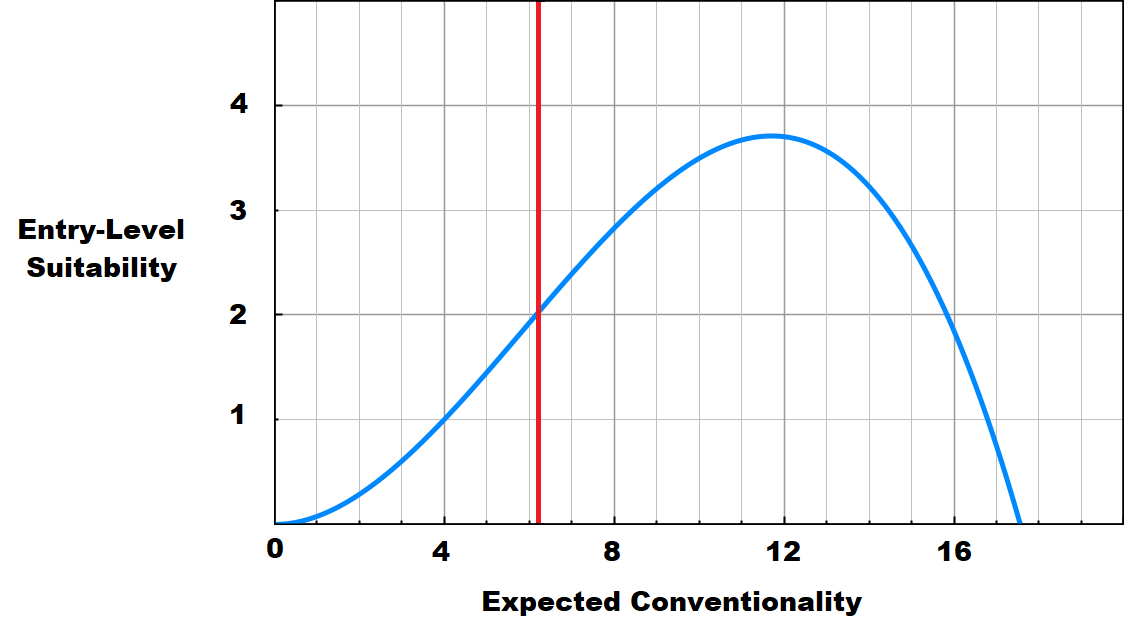
\includegraphics[width=0.7\textwidth]{./figures-and-tables/figure-3.png}};
                \node (n2) [above=0.25cm] at ($(n1)!0.5!(n1) - (6.2, 0)$) {\textbf{Suitability}};
                \node (n3) [above=0.25cm] at ($(n1)!0.5!(n1) - (0, 4)$) {\textbf{Expected Conventionality}};
        
                \end{tikzpicture}
        
            \label{fig:expect_convention_voi}
            \end{figure}
        
        The vertical line in Figure \ref{fig:expect_convention_voi} occurs at the mean value of expected conventionality, or about 6.1.
        Alternative credentials are past the lagged phase of adoption and recently past the
        point of inflection. Because expected conventionality cannot exceed a value of 10 by
        construction, the relation is isomorphic to a sigmoid over the range of actual values.
        Log-log regression of conventionalism on time obtains a p-value of .004.
        Expected conventionality is not binary,
        but a transformed variable was utilized for sigmoid modelling with logistic regression \cite{cox2008stata},
        Logistic regression obtained additional significance.
        
        Log-log, s-curve, and sigmoid relations are standard models for a variety of structurally important relationships.
        Social learning, experience, social influence, and contagion effects are some of the
        indicated structural relations\cite{young2009innovation}.
        Further identification of optimal fit may indicate effective accelerators of normalization.
        
        While the relationship between conventionality and time was strong,
        this is indirect to the variable of interest. Direct modelling of suitability
        on time was insignificant using logarithmic and logistic analysis, but
        a two-factor exponential expansion was discovered which forms a useful dynamic model:
        
        \begin{equation} f(x) = b_1b_2^t \end{equation}
        
        This nonlinear model obtained an r-squared of .8691 and $b_2$ had a p-value
        less than .001. The estimate of b2 was less than 1, indicating exponential
        decay rather than exponential growth. The data indicates a short-run reduction in entry-level
        suitability, with comparatively weak evidence for a reversal over time.
        
        When conventionality is interacted with time, a multiple regression suitability on time, conventionality, and the interaction
        reveals a positive relation between the interacted variable and suitability.
        This may point to long run normalization of alternative credentials as a mechanism toward eventual improvement in entry-level suitability.
        
        A simple interpretation is that employers are more pessimistic than others
        on alternative credentials. Another interesting possibility is that employer attitude is a leading indicator of population attitude.
        Nonlinear regression on time indicates a short-term decline in population favorability,
        which is consistent with employer-lead favorability, given that employers are more pessimistic than average in 2019 data.
        
        Exploring this notion, an interesting finding is identified using a multiple regression with interacted time and employer status.
        This regression of four parameters on the variable of interest is depicted in
        Figure \ref{fig:employer_driven_favorability}, which illustrates a hypothetical reversal in entry-level
        suitability. The figure is conceptual and not to scale. The population
        trend is illustrated at II, and employer views are represented at III. At II,
        time effects are linearly negative and marginally positive. Linear
        employer-time effects are positive, but marginal employer-time effects are
        negative. The plausibility of a reversal story is enhanced when noting
        that the coefficient of interacted manager-time is positive and large in magnitude compared to ordinary time effects.
        
        \begin{figure}[h!]
            \centering
            \caption{Employer Driven Favorability}
        
            \begin{tikzpicture}[element/.style={minimum width=1.75cm, minimum height=0.85cm}]
        
            \node (n1) [above=0.25cm] {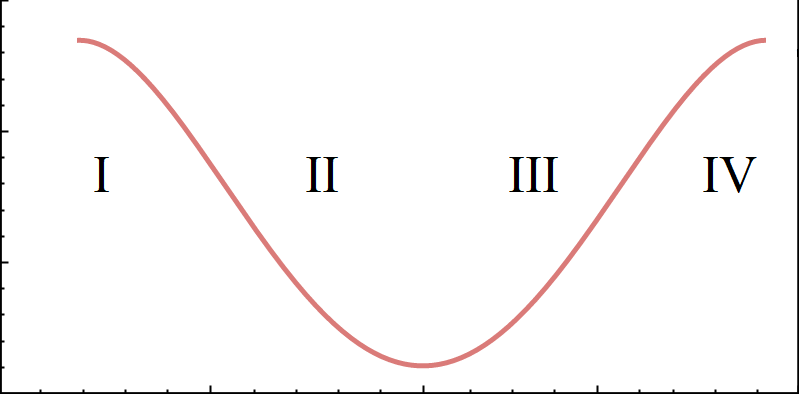
\includegraphics[width=0.7\textwidth]{./figures-and-tables/figure-4.png}};
            \node (n2) [above=0.25cm] at ($(n1)!0.5!(n1) - (6.2, 0)$) {\textbf{Suitability}};
            \node (n3) [above=0.25cm] at ($(n1)!0.5!(n1) - (0, 3.5)$) {\textbf{Time}};
        
            \end{tikzpicture}
        
            \label{fig:employer_driven_favorability}
            \end{figure}
        
        Age group had a more robust effect compared to exact age, which may
        indicate something like a cohort effect. Ethnic effects were moderately
        significant, and regional effects continued to be significant after the
        introduction of the ethnicity question in 2019, supporting the thesis
        that policy differences are important in this regard.
        
        Educational attainment obtained an important effect which was more
        significant than either age or income effects. In addition to level of
        education, a dummy variable for whether education was at or greater than
        obtaining a college degree was found to be significant. Increased
        education, whther traditional or non-traditional, appears to be
        associated with increased support for alternative credentials.
        
        % TODO: remove from concise paper
        \section{Other Interesting Results}
        
        Prior research finds student indifference toward debt\cite{davies1995student}.
        The present paper replicates and extends such
        findings to identify youth antagonism to alternative credentials. Prior
        research often measures debt attitudes among college students, but such
        evidence is susceptible to selection bias because debt-tolerant
        individuals might have a propensity to consume higher education. In
        contrast, the present paper identifies generalized youth antagonism to
        alternative credentials.
        
        In a simple regression, age has a small negative coefficient.
        Table \ref{tab:partial_crosstab_voi_agegroup} tells a more complex story.
        The most positive group is not the youngest group, but the age group actively
        attending or having just graduated college.
        
        \begin{table}
            \caption{Partial Crosstab of Age Group on Suitability}
            \begin{tabular}{lllllll}
                Suitability & $<$18 & 18-29 & 30-44 & 45-60 & 60$<$ & Total \\
                1 & 3 & 9 & 11 & 13 & 4 & 40 \\
                5 & 1 & 28 & 31 & 27 & 9 & 96 \\
                10 & 1 & 46 & 39 & 36 & 19 & 141 \\
                Total & 10 & 227 & 250 & 245 & 77 & 809 \\
                Average & 4.60 & 6.93 & 6.62 & 6.40 & 6.34 & 6.59 %
            \end{tabular}
            \label{tab:partial_crosstab_voi_agegroup}
            \end{table}
        
        Minors are the only age group which is unfavorable toward alternative credentials on average.
        Minors have the largest share of minimum-favorability responses.
        Minors are also the least sampled group in this data set.
        
        In the preferred model and several others, educational effects are important, including a
        dummy variable for having received a college-level or better education.
        One explanation is that participation in the traditional higher education
        drives support for alternative credentials, and the relationship with age is a
        side effect.
        
        An interesting, tangential result is the effect of nonbinary gender identification.
        Nonbinary gender identification, obtained for 16 respondents, was included in order to
        reduce noise on gender effects, but it turned out to have a significant independent effect.
        
        Simple regression of nonbinary gender identification on the variable of
        interest reveals a coefficient of about -1.3 with a p-value less than .05.
        Substituting nonbinary identification in for other gender variables in the strong model
        maintains the negative direction of effect, but the effect is
        attenuated to a coefficient of -.48 and a p-value of .374.
        
        % previously: \section{Applications}
        \section{Conclusions}
        
        Suppose that the average alternative learning program and the average traditional program
        provide equal benefit to a consumer, but suppose that alternative
        processes experience higher variance in consumer benefit. In this
        simple model we can see that the best programs would be alternative
        programs. Such a model can robustly predict that top programs are
        alternative, even when the alternative distrobution is modified such
        that the average alternative program is substantially worse than the
        average accredtied program.
        
        The extent of preference for alternative learning improves from
        occassional to usual once the simple model is extended to reflect the
        lower price and accelerated completion of alternative learning programs.
        For example, the price of a CLEP test is \$89 in 2019 dollars\cite{collegeboard_2019}, while
        the average cost per credit hour at an accredited college is \$594 in 2018
        dollars\cite{kirkham2018study}. A CLEP test may substitute for a 4-credit course\footnote{Credit
        may vary and is generally decided by the awarding institution rather than
        the exam provider. Other well-known credit by examination assessments include AP, Cambridge International, DSST, Excelsior
        College, and TECEP exams.}. This means credit by examination is approximately 15 percent of the price of credit by credit hour.
        Alternative learning programs may provide flexible financing options and greater earnings potential compared to a traditional program.
        
        % TODO: per youtube dude, placement rate has changed importantly over time
        % this may be related to shifting employer preference. underlying quality change
        General Assembly offers bootcamp-style education in several specific occupations. General Assembly
        charges \$14,950 for its priciest immersive course, but students
        can finance in creative ways. One option is to pay nothing upfront and utilize an income sharing
        agreement, so the student need not pay until employed full-time\cite{ga2019}.
        The immersive lasts about 3 months. For General Assembly
        full-time programs ending between July 1, 2014 and June 30, 2015, 88 percent of students found full-time
        work within 90 days of graduation, and 99 percent found full-time work within 180
        days\cite{kirkham_2017}. This is in notable contrast to the traditional degree, where 54 percent of
        the class of 2015 had found a standard, full-time job 6 months after
        graduation\cite{wexler_2016}.
        
        Bootcamps can sometimes be used as a college substitute, but they can also
        be used after college graduation to differentiate a job candidate from
        competitors, or to switch careers or brush up on recent changes
        mid-career. Finally, many traditional universities now offer through prior
        learning assessments or credit by portfolio, so that bootcamps can result
        in college credit even without officially partnering with a university\cite{aceposttraditionallearners}.

        % resumed from previously below
        
        Results have key applications for employers, students, and policy.
        Age results indicate an alternative credential marketing strategy targeted at
        current college students, recent graduates, and parents, rather than high school students.
        
        Employers tend to adopt practices supported by leaders in their own industry.
        This paper suggests that employers may be a leading indicator of broader attidudes.
        Given these two facts, a strategy for social adoption would be to target industry leaders.
        At the same time, we already see industry leaders disavowing the need for formal education.
        Glassdoor notes 15 leading companies, including Google, which no longer required a degree\cite{glassdoor_2018}. Glassdoor
        states, "Increasingly, there are many companies offering well-paying jobs
        to those with non-traditional education or a high-school diploma."
        
        % TODO: may not need this paragraph
        In 2013, Laszlo Bock, Senior Vice President at Google, stated that Google’s data at that time indicated
        that on the job performance was insignificantly related to GPA or test
        scores after 2-3 years, and the proportion of people without any college
        education at Google was increased over time\cite{bryant_2013}.
        
        For the corporate intrapreneur, direct appeal to industry leaders is one strategy.
        Another strategy is simply continued socialization of the topic within the organization.
        Results indicate that people are receptive to alternative education even if they aren’t
        familiar with the topic, and they become more favorable as they learn
        more\footnote{In a simple regression, respondents that know none of the available learning providers have predicted suitability at the model constant value of 6.4.
        Suitability moves positively with knowledge of additional alternative learning providers.
        Prima facie, this indicates that informing a person about alternative learning providers are expected to improve predicted suitability.}.
        A third strategy is to appeal to the underlying costs and benefits of an alternatively educated labor force.
        Alternatively educated students tend to be more diverse\cite{florentine_2018}, and improving diversity is often a corporate goal in itself.
        Alternatively educated students are also often willing to take a lower starting salary during the junior phase of their career, while providing similar or superior technical output.
        
        Students should consider conducting learning online, learning with non-elite providers,
        and leveraging credit by examination.
        For roles where a degree is inessential to junior placement, students should consider
        deferring college education until after industry employment is obtained.
        Once a student obtains employment in the industry, employers are often willing to pay the majority of a reasonably priced degree.
        This deferred degree strategy is a key way for a student to obtain a much better return on investment to their education than they otherwise would.
        Finally, students should consider leveraging digitial portfolios as a compliment to their degree,
        as a means of earning college credit through a prior learning assessment,
        and even as a substitute for the degree with respect to particular roles.
        
        Results for policymakers indicate redirecting or limiting federal grant and loan programs.
        Licenses which require formal education should be amended to support evidence-based competency in lieu of accredited education.
        Internship rules should be relaxed and the minimum wage should be frozen or reduced,
        to support better employment of young and concurrently learning individuals.
        Finally, tax write-offs and tax-privileged
        investment vehicles targeted at accredited education should be liberalized
        to support alternative education.
        
        % ref: https://www.youtube.com/watch?v=KS9GvK7cvmo
        % https://tex.stackexchange.com/a/51501/197312
        \bibliographystyle{./aea-latex-templates/aea}
        \bibliography{BibFile}
        
        \end{document}
        